\documentclass[11pt, twocolumn]{article}
\usepackage[total={6in, 8in}, margin=1.0in]{geometry}
\usepackage{booktabs} % for nice tables
\usepackage{longtable}
\usepackage{lmodern}
\usepackage{listings}
\usepackage{hyperref}
\usepackage{graphicx}
\usepackage{subcaption}
\usepackage{wrapfig}
\usepackage{cite}
\usepackage{url}
\usepackage{microtype}
\usepackage[toc,page]{appendix}
%\usepackage{lineno}

\usepackage{amssymb}
\usepackage{tabularx}
%\usepackage[paper=letterpaper,top=1in,bottom=1in,left=1in,right=1in]{geometry}

\usepackage[T1]{fontenc}
\usepackage[sc]{mathpazo}
\linespread{1.02}

\setlength\parindent{0pt}
\setlength{\parskip}{7pt plus4mm minus3mm}
\newcommand{\block}{\footnotesize $\blacksquare$ \normalsize}
%\pagestyle{empty}
\newcommand{\squeezeup}{\vspace{-5.5mm}}
%\linenumbers

\bibliographystyle{plain}

\begin{document}
\title{Bringing Spark and HPC to HEP Analysis}
\author{Saba Sehrish \\ Fermi National Accelerator Laboratory \\ ssehrish@fnal.gov}
\date{}
\maketitle

\thispagestyle{empty}

\section*{Abstract}
\squeezeup
Experimental HEP is a compute- and data-intensive statistical science. 
In our experience working with HEP scientists, it is repeatedly observed 
that interactive, iterative and low-latency analysis of PBs of data is the 
key to extract more science. HEP analysis is complex and consists of 
several steps that take from days to weeks to complete. We describe 
our experience of implementing an HEP analysis in Spark 
and evaluate its performance on HPC resources.

Track: Data Science  \\
Audience: Beginner, Intermediate technical talk \\
\squeezeup
\section{Introduction}
\label{sec:intro}
\squeezeup
HEP deals with the understanding of fundamental particles and the interactions between them.
Experimental HEP is a compute- and data-intensive statistical science; large number of interactions 
must be analyzed to discover new particles or to measure the properties of known particles. 
For example, data from over $300$ trillion ($3\times10^{14}$) LHC proton-proton collisions were analyzed for the Higgs boson discovery.
 %approximately $1$ in $10^{13}$ LHC collisions yielded a distinguishable Higgs boson~\cite{higgsboson1}. 
%The size of the data sample (25 petabytes per year) required the use of a worldwide computing grid, 
%comprised of 170 computing facilities across 42 countries~\cite{lhcgrid}. 
Future HEP experiments will bring in even more data, and processing and 
analyzing will be more challenging. For example, the LHC generates up to a billion collisions per second; the High Luminosity-LHC~\cite{hllhc} will generate 5 times this rate. These larger data samples will be needed to obtain a 
deeper understanding of the Higgs boson and its implications for the fundamental laws of nature. 
 
A typical HEP workflow to extract physics results from detector measurements consists 
of three steps; 
detector signal recording, data reconstruction, and data analysis. 
HEP detectors' data acquisition systems record detector signals and impose 
 a structure on the recorded data depending on the kind of detector and particle 
 interaction of interest. In the reconstruction step, physics quantities of broad interest 
(e.g., trajectories of charged particles) are extracted from raw instrument signals. 
The reconstruction step involves a variety of pattern recognition, clustering, and tracking algorithms. 
Reconstruction is normally performed on full raw data sets and is costly in terms of processing time.
Data analysis typically involves processing the reconstructed data using 
selection algorithms, calculations of statistical summaries, and exploratory plotting of the relevant summaries. 

%Experimental HEP extensively uses advanced analysis techniques and tools, including 
%multi-dimensional probability density estimation, 
%boosted decision trees, 
%and neural networks including deep learning neural networks~\cite{tmva, HEPadvana, deeplearninghiggs,deeplearninghep}. 

Running end user analyses that is needed for the next generation of HEP discoveries,  
has high latencies using current tools and resources, because of the large volume of data required. 
In this talk, we will present our
experience of implementing one use case from HEP; the CMS dark matter analysis, using Apache Spark~\cite{spark,spark1} and running tests at NERSC~\cite{nersc-spark}. Figure~\ref{fig:overview} summarizes our research focus. 
%!TEX encoding = UTF-8 Unicode\squeezeup
\begin{figure}[htbp]
\begin{center}
 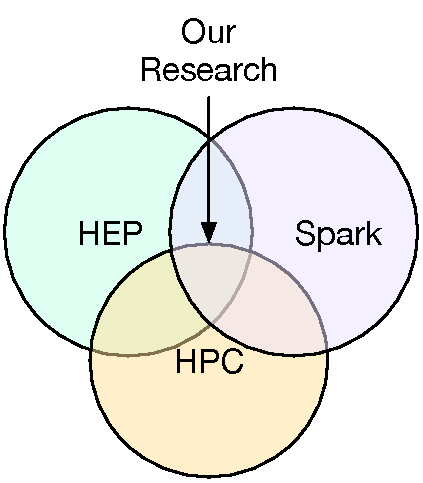
\includegraphics[scale=0.5]{overview}
\caption{The focus of our research}
\label{fig:overview}
\end{center}
\end{figure}
\squeezeup

\section{CMS Dark Matter Analysis}
This CMS Dark Matter analysis focuses on searching for new types of 
elementary particles. 
While most of these searches consist of attempting to detect astrophysical 
dark matter passing through detectors (direct searches), dark matter could 
also be produced in collisions at the Large Hadron Collider (LHC) if its 
constituent particles are of an appropriate mass. We carry out such a 
search using the CMS detector at the LHC. 

This CMS Dark Matter analysis is using composite C++ objects, 
which describes the analysis products of the reconstruction of either 
simulated or recorded collisions. 
The data volume is about 200 TB, and it takes about a week to form ntuples. 
 ntuples have a simple flat structure of vectors of basic types like integers and floats. 
%The analysis software framework BACON is used to produce ntuples. 
The ntuples undergo a process of skimming and slimming, and the data produced for this Dark Matter 
analysis use case is 2 TB. On average, this process is performed 
4 times a year, but can be executed much more frequent as needed. 
These ntuples are then used to analyze a specific channel of 
the Dark Matter analysis use case, many in parallel. 
The outputs of each team are plots and tables. 
It takes about 1 day to process all ntuples. 
A straight-forward approach is to simply count signal and background events, 
called cut-n-count. This is achieved by processing the ntuples 
and making optimized selection cuts. In the end, the required plots
 and tables are produced to extract the physics results of the analysis.
 Table~\ref{tab:1} shows different steps, input size and processing time. 
 The purpose of our study is to evaluate Spark for such analysis. 
%A more sophisticated approach is using machine learning techniques like multi-variate analysis approaches to separate signal and background. These require an intermediate step executed on subsets of the BACON ntuples to train the multi-variate technique and then apply it to the BACON ntuples. 

\begin{table}[h]
\begin{tabular}{ l | c | r }
\hline
  Steps & Input size & Processing time \\
  \hline
  Ntupling & 200 TB & ~ 1 week \\
  \hline
  Skimming \&  &2 TB  & ~ 1 day\\
  Slimming & & \\
  \hline
  Analysis &  << 1 TB & 5-30 minutes\\
  \hline
\end{tabular}
\caption{Input size and processing time for each step in 2015.}
  \label{tab:1}
  \end{table}

%Once:
%? Convert data and simulation into format suited for
%interactive analysis (NTuples)
%? Problem: too big for interactive analysis
%? Once or several times:
%? Skimming & Slimming: reduce number of events
%and information content
%? Analysts can explore data and simulation interactively
%? General requirements
%- Apply user queries on pre-calculated quantities
%- Add user-specified calculations ? use for selection as
%well

\squeezeup
\begin{figure}[htbp]
\begin{center}
 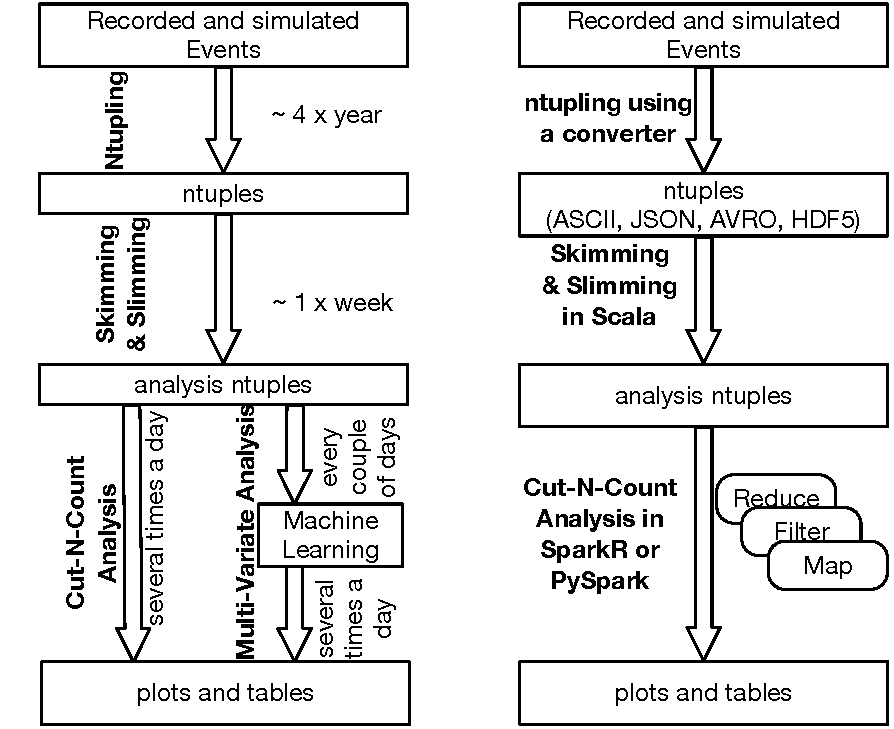
\includegraphics[scale=0.5]{flow}
\caption{Frequency of each step in current analysis and our approach to 
use Spark to implement each step. }
\label{fig:flow}
\end{center}
\end{figure}
\squeezeup

%\section{Approach}
%\squeezeup
%
%The input data is structured, and 
%2. Skimming and Slimming using Scala at large scale and ASCII and R at small scale
%3. Plots using SparkR

%\squeezeup
\section{Our approach using Spark}
\squeezeup
Spark allows for in-memory data processing, and is an attractive
approach for the cases where repeated analysis is performed on the
same data sets. A supported and tuned installation of Spark is
available at NERSC~\cite{nersc-spark}, and elimiates the need for 
the user to master the installation and tuning of the complex Spark system.
In the following discussion, we describe the pros and cons of using 
different features of Spark. Figure~\ref{fig:flow} shows the mapping of 
different steps in current analysis to the Spark framework. The conversion 
step is extremely important because the structure of data defines 
what APIs can be used later on in the Cut-N-Count analysis. 

\begin{enumerate}
\item \textit{Input data format: } 
The first step to implement our use case in Spark is to convert the data in the form that 
can be readily read in Spark DataFrames using native API as shown in Figure~\ref{fig:flow}. 
The CMS data is stored in the form of ROOT trees~\cite{root}, which is the most common 
data format in HEP but not accessible in Spark. 
This data format is hierarchical and complex. Initially data is converted to either 
JSON or ASCII for experimentation with sparkR and PySpark. 
The nested object structure of the data made it extremely inconvenient to read 
any data using the current API both with sparkR and pySpark. 
Hence, we need a flattened table to effectively use the API. 
Additionally, we are working to use AVRO and HDF5 data formats for the production. 
The use of HDF5 will be extremely useful as it is one of the tuned and supported 
parallel I/O libraries available on HPC machines. 

\item \textit{Operations on multiple DataFrames: } 
Currently we read data in multiple logical tables, e.g. every information regarding 
electrons can be in one table, etc. The nature of analysis is to combine the data from different tables 
and make several histograms for different particles. 
In our experience, if we read data in multiple DataFrames, 
adding a new column to the DataFrame from another 
DataFrame is not supported in Spark. Spark only supports adding new columns within the same DataFrame. 
In order to address the previous hurdle we attempted to use inner join, but the overhead of the 
\texttt{join} operation is extremely overwhelming that we are considering to pre-process the data, and 
make amendments to data files before copying data to NERSC. 

\item \textit{Spark Operations and scaling: } 
This analysis requires skimming and slimming operation; Scala is a natural choice 
to implement this operation; Spark is written in Scala, python will perform slow with large data sets.  
The skimming and slimming operation involves the use of functions; \texttt{map}, \texttt{filter} and 
\texttt{reduce}. 
We have used Java in our initial study to perform filter and reduction 
operation and understand the performance and scaling. Using a data set of size 250 GB, 
with about 70 million events and applying a simple filter operation, 
the Spark implementation provided good
  scaling without requiring any tuning to the implementation and
  developer expertise in parallel algorithms. 
  %However, we are working to understand the performance.  

\item \textit{Orchestration: } 
In Spark, data distribution and task assignment
  is abstracted from the user. There are functions available to
  perform global reduction in a distributed environment, which can be
  readily used.  Such a set-up provides ease-of-programming in a
  distributed environment. It does mean, however, that the user has to
  rely on system optimizations provided by Spark's implementation to
  improve any performance.
% Spark provides implicit parallelization of the
%physicists' data processing algorithms, thus providing the possibility
%of good scaling to large numbers of cores without requiring the
%physicists to master complex parallel programming techniques. This
%provides important ease of use for ``casual'' programmers, for whom
%the goal is rapid performance of analysis, who are usually not
%interested in developing specialized parallel programming
%skills.  
% 
\item \textit{Application tuning: } All the transformations in Spark
  are lazy, with delayed calculation of results. The transformations
  applied to the base dataset e.g. a file are remembered by the system
  and only computed when an action is carried out on the dataset.
  This design enables Spark to run more efficiently. 
%  For example, it
%  can recognize that a dataset created through \texttt{map} will be
%  used in a reduce and return only the result of the reduce to the
%  driver, rather than the larger mapped dataset. 
  Due to this lazy evaluation, it is hard to isolate slow-performing tasks and report
  timing for different stages. 

%\item \textit{Wrapped types: } We used the Java DataFrame API, and
%  most of the available operations for our implementation are
%  available through the Java wrapped types. A lot of time was spent in
%  boxing and unboxing.  It is well known that wrapped types perform
%  much slower than the primitive types, as explained in
%  ~\cite{effectivejava}. ``... Changing the declaration of sum from
%  Long to long reduces the run-time from 43 seconds to 6.8 seconds on
%  my machine. The lesson is clear: prefer primitives to boxed
%  primitives, and watch out for unintentional autoboxing
%  ...''~\cite{effectivejava}.  We did a test on Cori to compare the
%  performance of Float and float by running a simple Java program
%  based on the calculations of the classification algorithm, and
%  observed a performance difference of $28\%$ in using unboxed types.
%  Hence, we can achieve better performance with Spark if DataFrames
%  used primitive types.
%%[Boxed type test on Cori? 23 sec Vs 1 min 20 sec. ]
%
%
%\item \textit{Vectorized linear algebra library: } We experienced slow
%  performance for repetitive numerical computations in Spark due to
%  unavailability of high performance linear algebra library.  In the
%  MPI implementation, we used Armadillo, which is a high quality C++
%  linear algebra library.  The use of advanced libraries without data
%  conversions, and the ability to use vectorized hardware allowed MPI
%  implementation to perform exceedingly well as compared with Spark.

\end{enumerate}
\squeezeup
\textbf{Participation}: I will attend the conference. 

\textbf{Bio:} 
Saba Sehrish is a Computer Science Researcher 
at Fermilab. Prior to that she was a post doc at Northwestern University, 
and did her PhD from University of Central Florida. 
Her research interests include HPC and Big data computing for HEP analysis.  
She is currently working on Spark and also a team member of the LArSoft 
project at Fermilab. 

\textbf{Collaborators: } 
Matteo Cremonesi, Oliver Gutsche, Jim Kowalkowski, 
Cristina Mantilla, Marc Paterno, Jim Pivarski, Alexey Svyatkovskiy
\squeezeup
\scriptsize

%Bibliography and References Cited
\bibliography{earlycareerbib,ssio}

\end{document}
